\chapter{Análise e Discussão dos Resultados}
\label{cap:results}

Com base nos resultados obtidos na pesquisa aplicada aos empresários/gestores, caracterizados como público alvo, foi feita a análise dos dados, buscando a correlação dos fatores habilitadores identificados com as características de empresas que possuem um tempo de atuação no mercado considerado acima da média. 

\section{Análise dos resultados}
\label{subsec:framing}

Do total de empresas que comercializam produtos/serviços on-line, 94,9\% foram representadas por PMEs e 5.1\% por startups. Essas empresas relataram em sua maioria que preferem divulgar/comercializar seus produtos/serviços nas redes sociais com 87.5\%, seguido pela escolha do marketplace, com 60\%, como mostrado na Figura \ref{fig:plataformas}.

% Imagem fixa
\begin{figure}[h]
 
\centering
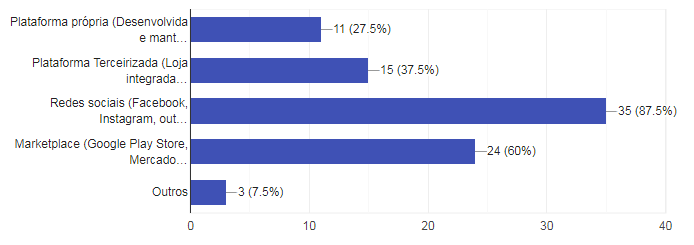
\includegraphics[width=14cm]{./fig/plataformasusadas}
\caption{Plataformas que as empresas divulgam/comercializam produtos/serviços on-line. (Fonte: Autoria própria, 2019)}
\label{fig:plataformas}
\end{figure}

A maioria da empresas consultadas na pesquisa possuem de 1 a 6 anos de atuação no mercado, representando 33,3\%, logo após temos as empresas com até 1 ano de atuação, com 28,2\%. As organizações com mais de 6 anos de atuação, representaram 25,6\% do total de entrevistados. Os gestores em sua maioria, informaram possuir nível de conhecimento em tecnologia da informação considerado razoável, com 46,2\%, como mostrado na figura \ref{fig:tempodemercado}. 

% Duas imagens -------------
\begin{figure}[H]
\center
\subfigure[08][Tempo de mercado.]{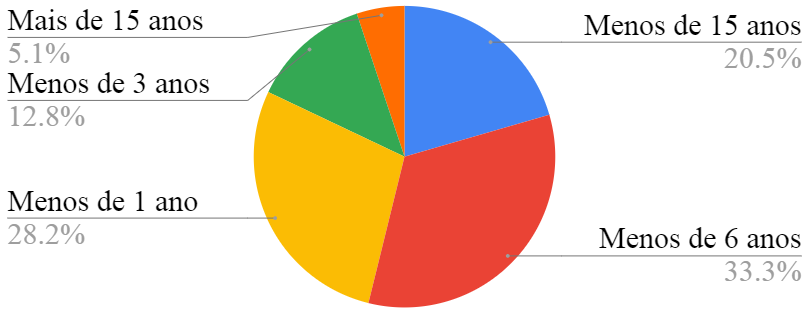
\includegraphics[width=7cm]{./fig/idade}}
\qquad
\subfigure[10][Nível de conhecimento em tecnologia da informação.]{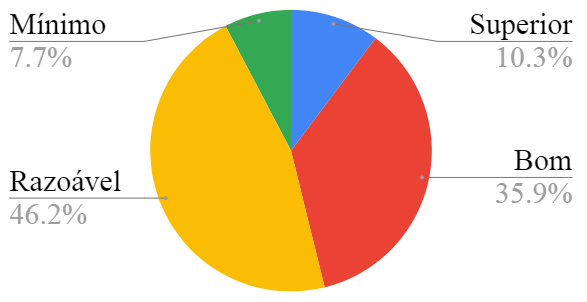
\includegraphics[width=5.5cm]{./fig/conhecimentoemti}}
\caption{Questões 8 e 10. (Fonte: Autoria própria, 2019)}
\label{fig:tempodemercado}
\end{figure}

As empresas em sua maioria terceirizam alguma função específica, recurso ou infraestrutura de TI, representando 61,5\%, o restante, 38,5\% optam por não tercerizar. A maior parte delas, 64,1\%, informaram que não utilizam o método cross docking para o gerenciamento de estoque de sua empresa, o que já era esperado, pois a maioria delas atua no mercado de desenvolvimento de software e na área de prestação de serviços.

Grande parte das empresas, representando 56,4\%, relataram que mapeiam o perfil do consumidor e atuam em um mercado de nicho, segmentado. Os empresários/gestores entrevistados, em sua maioria, com 61,5\%, realizam a análise ambiental e promovem estudos de redesenho (pivotar) dos processos da empresa regularmente.

Dentre as organizações, 59\% informaram que utilizam algum instrumento indicador que monitora e acompanha o nível de desempenho (KPIs, satisfatório, ou insatisfatório) e o nível de atingimento dos objetivos organizacionais (KRIs), 41\% não utilizam instrumento indicador em sua empresa. A maioria das empresas consultadas, 72,5\%, não estão inseridas em alguma comunidade empresarial, seja ela cooperativa ou associativa.

A maior parte das organizações, com 79,5\%, atuam na criação de conteúdo relevante e o distribui em redes sociais e campanhas de e-mail marketing. 61,5\% dos entrevistados fazem o acompanhamento durante o período de pós-venda, monitorando o feedback dos clientes na internet, tanto em redes sociais como sites de reclamação, para poder melhorar um produto/serviço.

Foi constatado que as pessoas que possuem nível de conhecimento em tecnologia da informação “Bom” ou “Superior”, estão, em sua maioria em empresas que possuem maior tempo de mercado, ou seja, acima de 3 anos de atuação. A maioria das pessoas que declaram possuir nível de conhecimento em tecnologia da informação “razoável” estavam presentes em empresas com menos de 1 ano de atuação. As empresas com mais de 15 anos de atuação possuem pessoas com nível de conhecimento em tecnologia da informação considerado “bom”, conforme a figura \ref{fig:grafico48}.

% Imagem fixa
\begin{figure}[H]

\centering
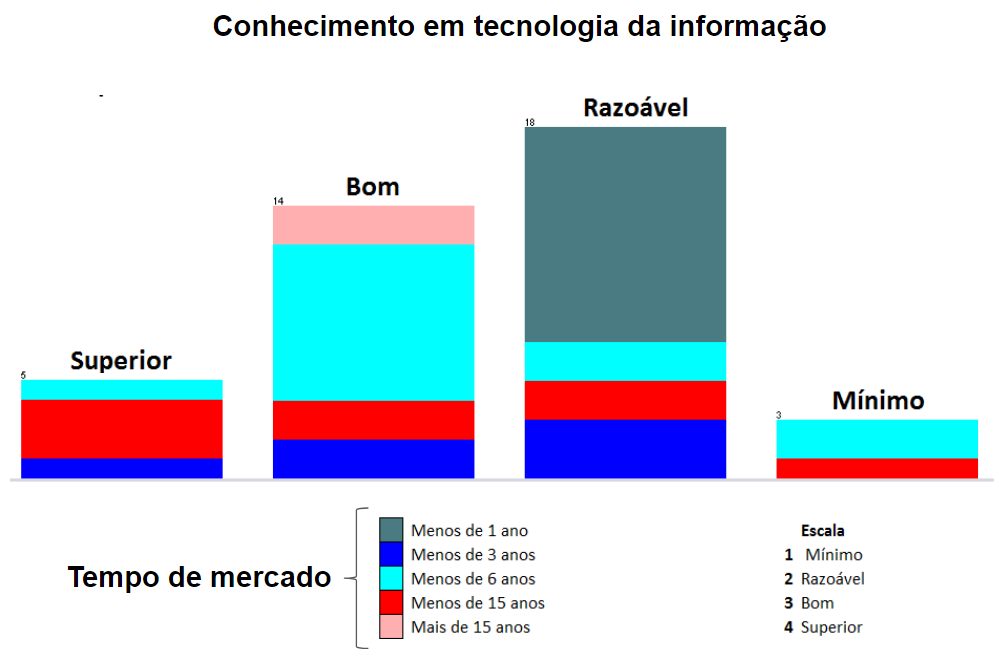
\includegraphics[width=13cm]{./fig/grafico01}
\caption{Conhecimento em TI X Tempo de mercado. (Fonte: Autoria própria, 2019)}
\label{fig:grafico48}
\end{figure}

As empresas que utilizam algum instrumento indicador que monitora e acompanha o nível de desempenho (KPIs, satisfatório, ou insatisfatório) e o nível de atingimento dos objetivos organizacionais (KRIs) são as que possuem maior tempo de mercado. As empresas com menos de 1 ano de atuação estão em sua maioria no grupo que não utilizar nenhum instrumento indicador, conforme mostrado na figura \ref{fig:grafico49}.

% Imagem fixa
\begin{figure}[H]

\centering
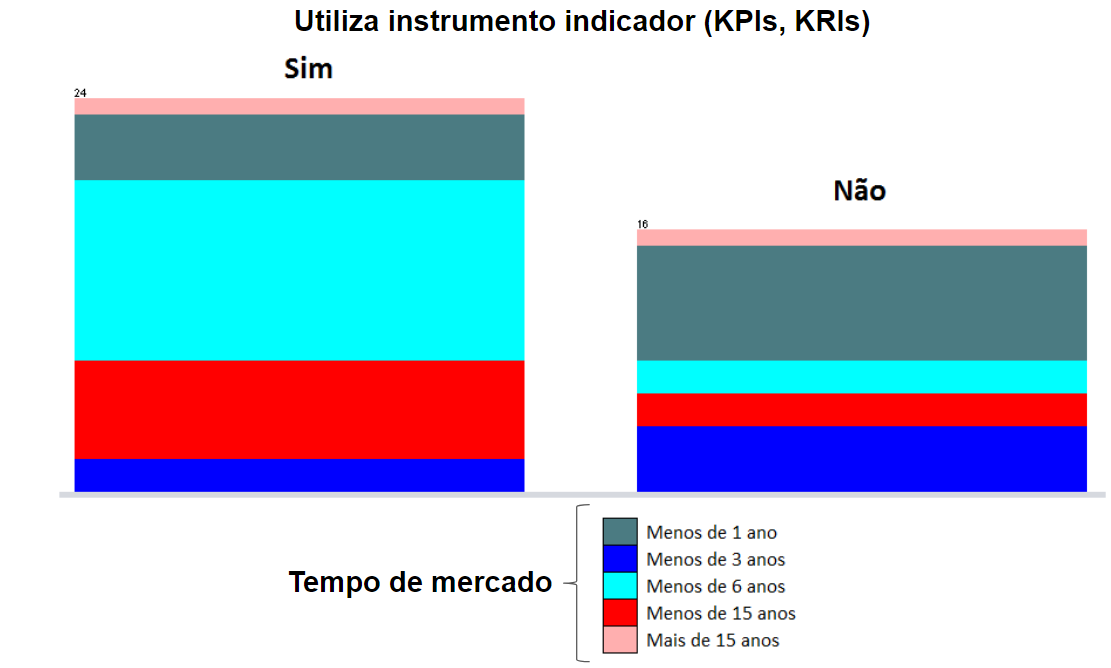
\includegraphics[width=13cm]{./fig/grafico05}
\caption{Utiliza instrumento indicador (KPIs, KRIs) X Tempo de mercado. (Fonte: Autoria própria, 2019)}
\label{fig:grafico49}
\end{figure}

As pessoas que informaram possuir nível de conhecimento em tecnologia da informação “Superior” utilizam algum instrumento indicador (KPIs, KRIs) em sua empresa, como demonstrado na figura \ref{fig:grafico411}. Todos os entrevistados que possuem nível de conhecimento em TI “mínimo” não utilizam instrumento indicador (KPIs, KRIs) em suas empresas.

% Imagem fixa
\begin{figure}[H]

\centering
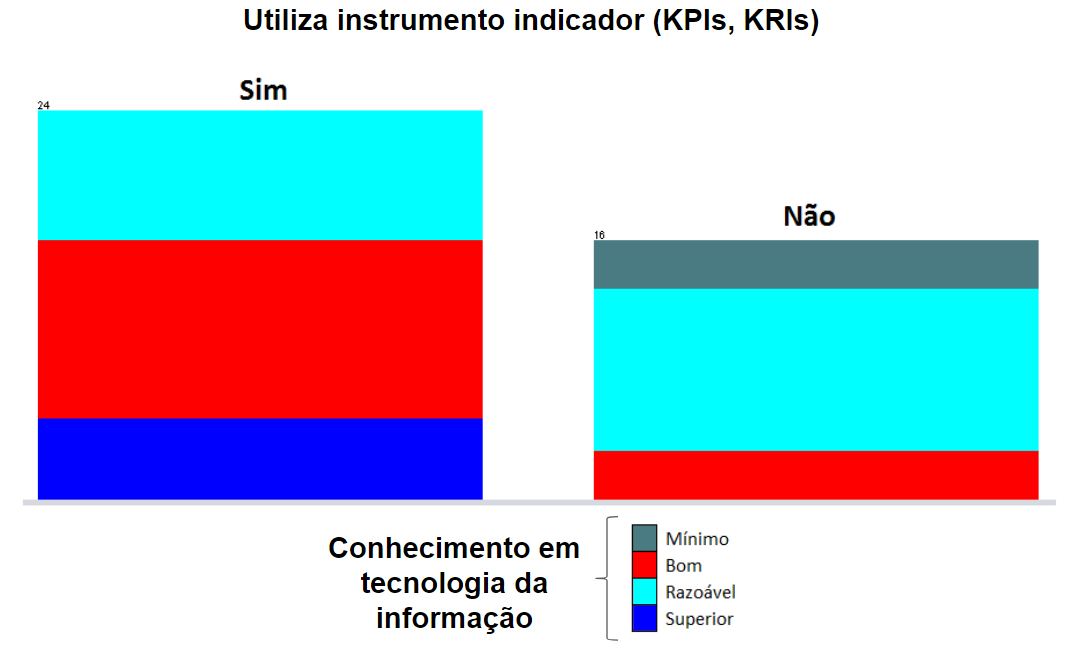
\includegraphics[width=13cm]{./fig/grafico08}
\caption{Utiliza instrumento indicador (KPIs, KRIs) X Conhecimento em TI. (Fonte: Autoria própria, 2019)}
\label{fig:grafico411}
\end{figure}

As pessoas com nível de conhecimento em TI “Superior” estão presentes no grupo que cria conteúdo relevante e o distribui em redes sociais e campanhas de e-mail marketing, como descrito na figura \ref{fig:grafico412}. Por outro lado, a maioria das pessoas com nível de conhecimento em TI “mínimo” não cria conteúdo relevante e o distribui em redes sociais e campanhas de e-mail marketing. 

% Imagem fixa
\begin{figure}[H]

\centering
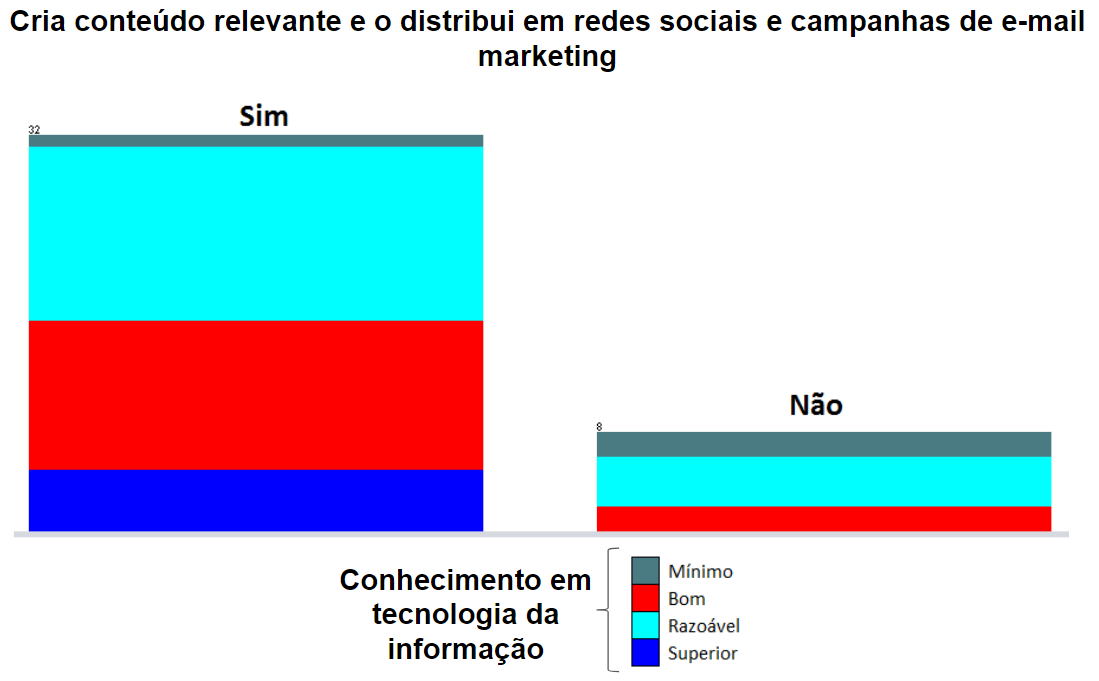
\includegraphics[width=13cm]{./fig/grafico09}
\caption{Cria conteúdo relevante e o distribui em redes sociais e campanhas de e-mail marketing X Conhecimento em TI. (Fonte: Autoria própria, 2019)}
\label{fig:grafico412}
\end{figure}

Na figura \ref{fig:grafico410} é mostrado que as empresas com maior tempo de mercado, em sua maioria, fazem o acompanhamento durante o período de pós-venda, monitorando o feedback dos clientes na internet, tanto em redes sociais como sites de reclamação, para poder melhorar um produto/serviço. Já as empresas com menos de 1 ano de atuação não fazem esse acompanhamento.

% Imagem fixa
\begin{figure}[H]

\centering
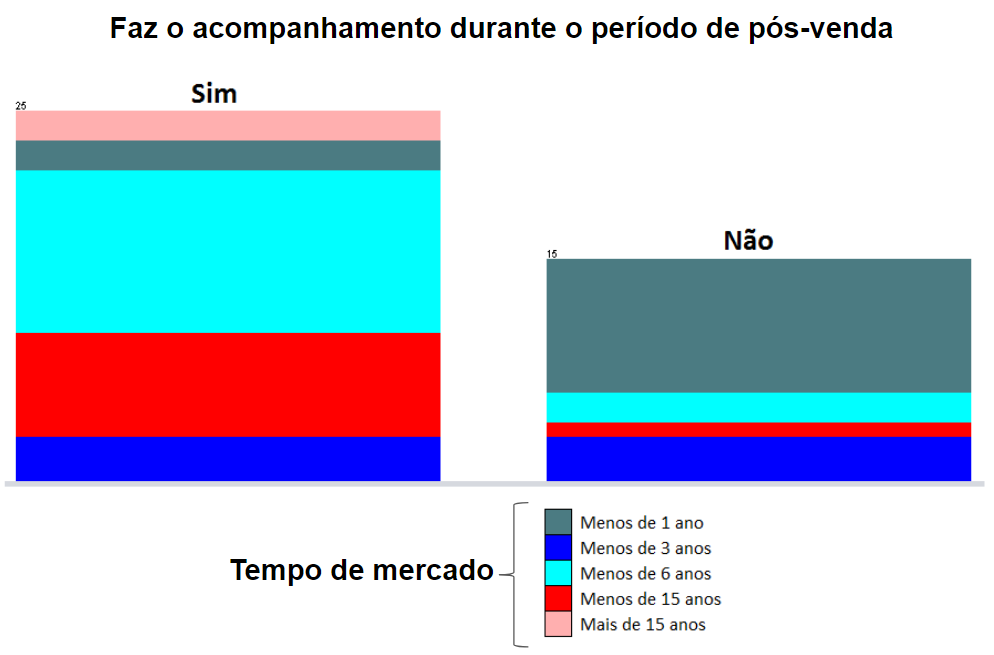
\includegraphics[width=13cm]{./fig/grafico06}
\caption{Faz o acompanhamento durante o período de pós-venda X Tempo de mercado. (Fonte: Autoria própria, 2019)}
\label{fig:grafico410}
\end{figure}

Na figura \ref{fig:grafico413} podemos ver a comparação das variáveis  “empresas que terceirizam alguma função específica, recurso ou infraestrutura de TI”, representado pelas duas colunas e “empresas que realizam a análise ambiental e promovem estudos de redesenho dos processos” representado pelas cores azul e vermelho. A pesquisa mostrou que a maioria das empresas que terceirizam alguma função específica, recurso ou infraestrutura de TI, realizam a análise ambiental e promovem estudos de redesenho dos processos. 

% Imagem fixa
\begin{figure}[H]

\centering
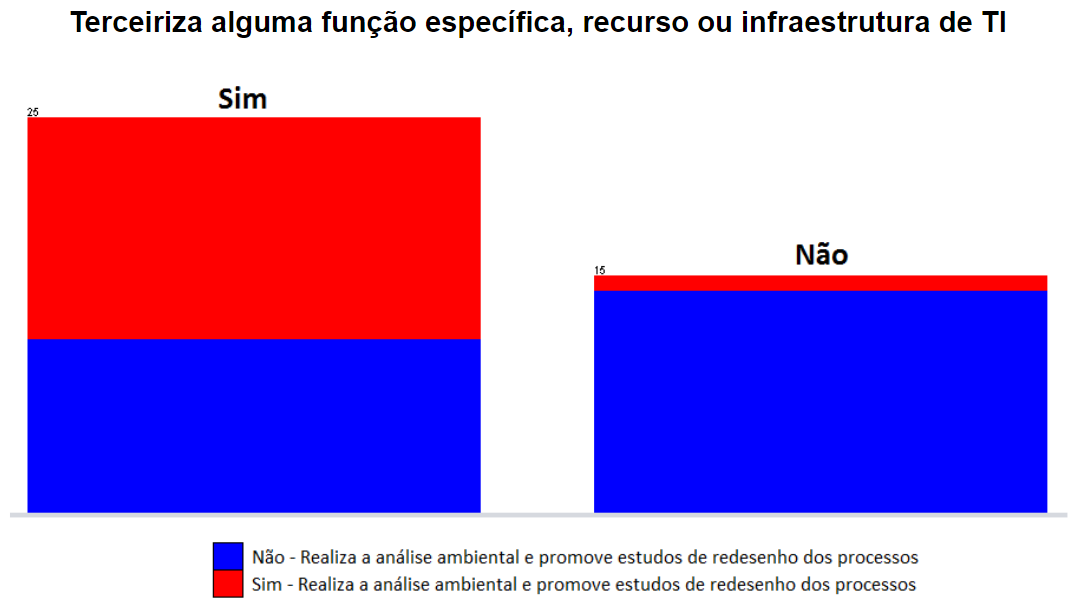
\includegraphics[width=13cm]{./fig/grafico11}
\caption{Terceirização e estudos de redesenho dos processos. (Fonte: Autoria própria, 2019)}
\label{fig:grafico413}
\end{figure}
	
Conforme a figura \ref{fig:grafico414}, foi identificado que as empresas que realizam a análise ambiental e promovem estudos de redesenho dos processos também utilizam, em sua totalidade, algum instrumento (indicador)  que monitora e acompanha o nível de desempenho (KPIs, satisfatório ou insatisfatório) e o nível de atingimento dos objetivos organizacionais (KRIs).

% Imagem fixa
\begin{figure}[H]

\centering
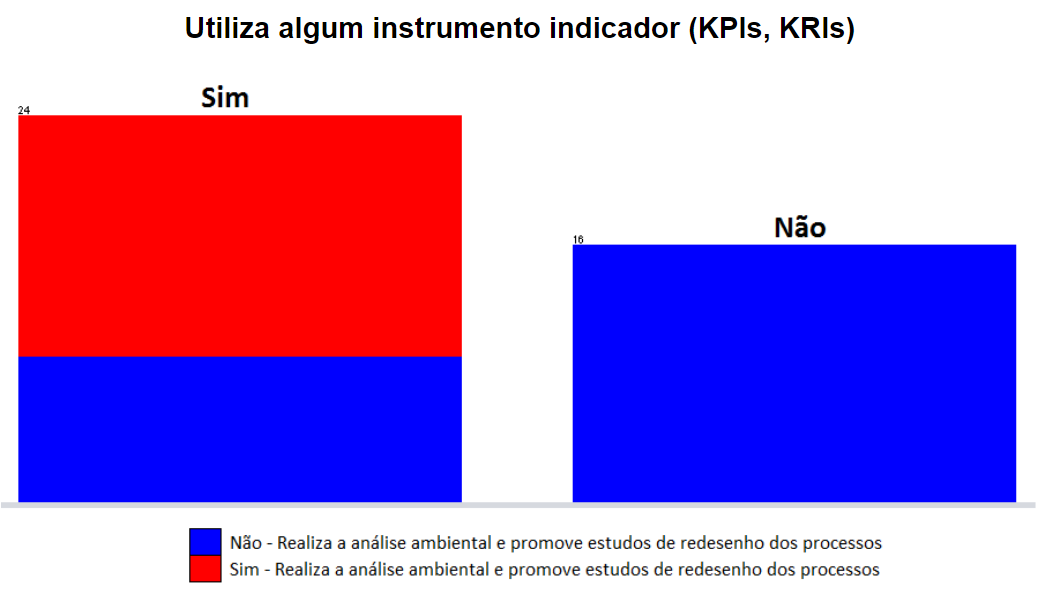
\includegraphics[width=13cm]{./fig/grafico12}
\caption{Utiliza algum instrumento indicador (KPIs, KRIs) X Promove redesenho dos processos. (Fonte: Autoria própria, 2019)}
\label{fig:grafico414}
\end{figure}


\section{Discussão dos resultados}
\label{subsec:framing}

Através dos dados, observa-se que as pessoas que possuem nível de conhecimento em tecnologia da informação “Bom” ou “Superior”, estão, em sua em sua maioria em empresas que possuem maior tempo de atuação no mercado, o que evidencia que o fator habilitador “conhecimento em tecnologia da informação”, citado na seção \ref{subsec:conhecimentoti}, exerce influência nas empresas que atuam de forma eletrônica.

As empresas que utilizam algum instrumento indicador que monitora e acompanha o nível de desempenho (KPIs, satisfatório, ou insatisfatório) e o nível de atingimento dos objetivos organizacionais (KRIs) são as que possuem maior tempo de atuação no mercado. Essa informação reforça a tese de que o fator habilitador “indicador de desempenho”, citado na seção \ref{subsec:kpi} deste estudo, contribui para um resultado satisfatório da organização. Efetuar a gestão da empresa utilizando indicador de desempenho (KPIs, KRIs) será um diferencial competitivo, e um fator crucial para a sobrevivência e crescimento no cenário em que a concorrência está cada vez maior e os clientes mais exigentes.

As pessoas que informaram possuir nível de conhecimento em tecnologia da informação “Superior” utilizam algum instrumento indicador (KPIs, KRIs) em sua empresa, essas pessoas também estão presentes no grupo que cria conteúdo relevante e o distribui em redes sociais e campanhas de e-mail marketing. O que mostra que, quanto maior o conhecimento em TI, presente nos empresários/gestores, mais habilitado estará essa organização para tomar decisões, seja para utilizar novas ferramentas ou manipular as que já existam na organização.

De acordo com a pesquisa, a maioria das empresas com menos de 1 ano de atuação não fazem o acompanhamento durante o período de pós-venda, monitorando o feedback dos clientes na internet, tanto em redes sociais como sites de reclamação, para poder melhorar um produto/serviço, como dito pelo Sebrae, na seção \ref{sec:vidautil}, que as empresas são iniciadas com falta de planejamento e deficiências de gestão. 

A maioria das empresas com mais de 3 anos de atuação no mercado faz o acompanhamento durante o período de pós-venda, monitorando o feedback dos clientes na internet, tanto em redes sociais como sites de reclamação, para poder melhorar um produto/serviço. Desta forma, é evidenciado que o fator habilitador “melhoria contínua”, seção \ref{subsec:bpr}, pode influenciar de forma positiva uma organização.

As empresas que realizam a análise ambiental promovendo estudos de redesenho dos processos, em sua maioria, são as que terceirizam alguma função específica, recurso ou infraestrutura de TI, descrito na seção \ref{subsec:terceirizacao}. O que mostra que as empresas que possuem o fator “melhoria contínua”, citado na seção \ref{subsec:bpr}, optam por terceirizar alguma função/recurso e assim se dedicar a outras atividades chave. A terceirização pode melhorar o desempenho das empresas que não têm conhecimentos ou não querem gastar seus recursos internos em certas áreas.

